\documentclass[11pt,a4paper]{article}
\usepackage[top=3cm, bottom=2cm, left=3cm, right=2cm]{geometry}
\usepackage[utf8]{inputenc}
% \usepackage[T1]{fontenc}
\usepackage{amsmath, amsfonts, amssymb}
\usepackage{siunitx}
\usepackage[brazil]{babel}
\usepackage{graphicx}
\usepackage[margin=10pt,font={small, it},labelfont=bf, textfont=it]{caption}
\usepackage[dvipsnames, svgnames]{xcolor}
\DeclareCaptionFont{MediumOrchid}{\color[svgnames]{MediumOrchid}}
\usepackage[pdftex]{hyperref}
\usepackage{natbib}
\bibliographystyle{plainnat}
\bibpunct{[}{]}{,}{s}{}{}
\usepackage{color}
\usepackage{footnote}
\usepackage{setspace}
\usepackage{booktabs}
\usepackage{multirow}
\usepackage{subfigure}
\usepackage{fancyhdr}
\usepackage{leading}
\usepackage{indentfirst}
\usepackage{wrapfig}
\usepackage{mdframed}
\usepackage{etoolbox}
\usepackage[version=4]{mhchem}
\usepackage{enumitem}

\setlist[itemize]{label=\textcolor{CarnationPink}{$\mathbf{\square}$}}

\setlist[enumerate]{label=\textcolor{CarnationPink}{\arabic*.}, align=left}


\newcounter{exemplo}

\NewDocumentEnvironment{exemplo}{ O{} }{%
\allowbreak
\setlength{\parindent}{0pt}
  \begin{mdframed}[
  leftline=true,
  topline=false,
  rightline=false,
  bottomline=false,
  linewidth=2pt,
  linecolor=CarnationPink,
  frametitlerule=false,
  frametitlefont=\Large\bfseries\color{CarnationPink},
  frametitle={\color{CarnationPink}\normalfont\bfseries #1},
  ]
}{%
  \end{mdframed}
}

\setlength{\fboxsep}{10pt}
\setlength{\fboxrule}{1pt}
\usepackage{float}
\renewcommand{\thefootnote}{\alph{footnote}}
\usepackage{url}
\hypersetup{
    colorlinks=true,
    linkcolor=cyan,
    filecolor=cyan,      
    urlcolor=cyan,
    citecolor=cyan,
    pdftitle={Resumos}
}
\pagestyle{fancy}
\fancyhf{}
\renewcommand{\headrulewidth}{0pt}
\rfoot{Página \thepage}

\title{Dosimetria}
\author{Detectores de Radiação\nocite{*}}
\date{\textit{Dalila Mendonça}}
\begin{document}
	\maketitle

\section{Propriedades Gerais dos Detectores de Radiação}

    Um detector quando submetido à radiação, terá um volume que será responsável por detectar a radiação e efetuar a leitura. Quando a radiação interage com o volume do detector, ela irá causar ionizações, ou seja, arrancará um elétron do átomo inicialmente neutro, e fará com que seja formado um par elétron íon, cargas negativas e cargas positivas. A interação ou o total freamento da partícula ocorre em um tempo muito curto, o que permite dizer que a deposição de energia é feita instantaneamente. 

    Assumindo a interação devido a apenas um quanta de energia (uma única partícula), a carga gerada dentro do detector ocorrerá então no tempo $t = 0$ (instantâneo). Na sequência, a carga deverá ser coletada na forma de sinais elétricos, cujo processo de detecção normalmente está acompanhado de um campo elétrico interno, que faz com que as cargas positivas e negativas se movam em direções opostas. 

    O tempo para coletar todas as cargas formadas nos detectores varia de um tipo de detector para outro, por exemplo as câmaras de ionização o tempo para coletar todas as cargas é da ordem de poucos milissegundos, enquanto que o tempo de coleção dos  diodos semicondutores é da ordem de poucos nanossegundos. Esses tempos de coleta estão relacionados à mobilidade dos portadores de carga e também à distância que os portadores de carga percorrem até serem coletadas no eletrodo coletor.

    Portanto, para a interação de apenas um quanta de energia, a resposta do detector será uma corrente que flui por um tempo igual ao tempo de coleta da carga. A figura \ref{fig:esquemaTempoColetaCorrente} mostra uma possível dependência temporal da corrente do detector, onde $t_c$ é o tempo para coletar a carga;

        \begin{figure}[h]
            \centering
            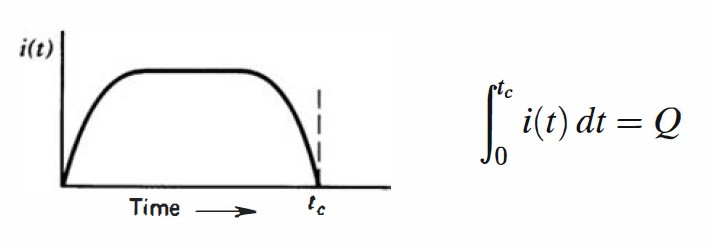
\includegraphics[width=0.7\textwidth]{Imagens/esquemaTempoColetaCorrente.jpg}
            \caption{Corrente em função do tempo de coleta da carga}
            \label{fig:esquemaTempoColetaCorrente}
        \end{figure}

	\noindent A integral da corrente ao longo de todo o tempo de coleta é igual quantidade total de carga gerada naquela interação específica. 

	Em situações reais, vários quantas estão interagindo com o volume do detector ao longo de um período de tempo. Portanto, para os casos em que há uma alta taxa de irradiação, a corrente gerada pode ser devida a mais de uma interação.  Assumindo que o detector está submetido a uma baixa taxa de radiação, de forma que cada interação irá gerar uma corrente que pode ser distinguida das demais interações. A medida que cada interação ocorre, serão gerados pulsos de correntes elétricas de modo que a intensidade de duração do pulso de corrente poderá variar dependendo do tipo de interação. A Figura \ref{fig:esquemaCorrentePulsada} mostra um esquema da corrente elétrica instantânea fluindo no detector ao longo do tempo.

		\begin{figure}[h]
			\centering
			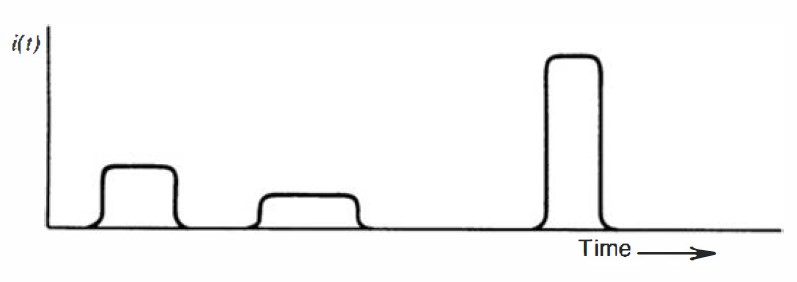
\includegraphics[width=0.7\textwidth]{Imagens/esquemaCorrentePulsada.jpg}
			\caption{Esquema de Pulsos de Corrente ao longo do tempo de medição do detector}
			\label{fig:esquemaCorrentePulsada}
		\end{figure}

	\noindent Pode-se observar diferentes intensidades de corrente e diferentes tempos de coleta de cada pulso. Nota-se também que, como a emissão de radiação é um processo aleatório, os intervalos de tempo entre um pulso de corrente e outro também é aleatoriamente distribuído. 
      
	\subsection{Modos de Operação Dos Detectores}

		Existem três modos de operação dos detectores, \textcolor{CarnationPink}{\textbf{\textit{Modo Pulso, Modo Corrente e Modo de tensão quadrada média (MSV)}}}; ambos operam de forma diferente e estão inter-relacionados através de suas dependências com as sequências de pulsos de correntes geradas no detector. 

		Como a energia depositada no detector é diretamente relacionada com a carga total $Q$ geradas através das interações dos quantas de energia com o detector, é de interesse que todas as cargas sejam coletadas e portanto o instrumento de medição irá operar no \textcolor{CarnationPink}{modo pulso} de forma que toda interação individual seja registrada. 

		O \textcolor{CarnationPink}{modo pulso} também é utilizado nos \textcolor{CarnationPink}{contadores de pulsos}, que se enquadra naquelas situações onde não é de interesse registrar a distribuição de energia da radiação, ou seja, não é de interesse obter energia depositada pelos quantas de radiação, o interesse é apenas obter a intensidade da radiação incidente; Para estes casos, é estabelecido um limiar de baixo nível para os pulsos gerados de forma qua qualquer pulso de corrente acima deste limiar é registrado pelo detector, independente do valor de Q.

		O \textcolor{CarnationPink}{modo corrente} e o \textcolor{CarnationPink}{modo MSV} são utilizados naquelas situações em que a taxa radiação é muito alta de forma que o modo pulso seja impraticável pois o tempo entre eventos adjacentes é muito pequeno de forma que não seja possível realizar uma análise adequada da carga coletada e os pulsos de corrente gerados podem se sobrepor ao longo do tempo; Sendo necessário, então, utilizar instrumentos de medição que respondem à media de tempo no qual ocorrem muitos eventos individuais;

		\subsubsection{Modo Corrente}

			A Figura \ref{fig:esquemaModoCorrente} apresenta o esquema de um detector operando no modo corrente, onde um amperímetro é conectado aos terminais de saída do detector de radiação;

				\begin{figure}[h]
					\centering
					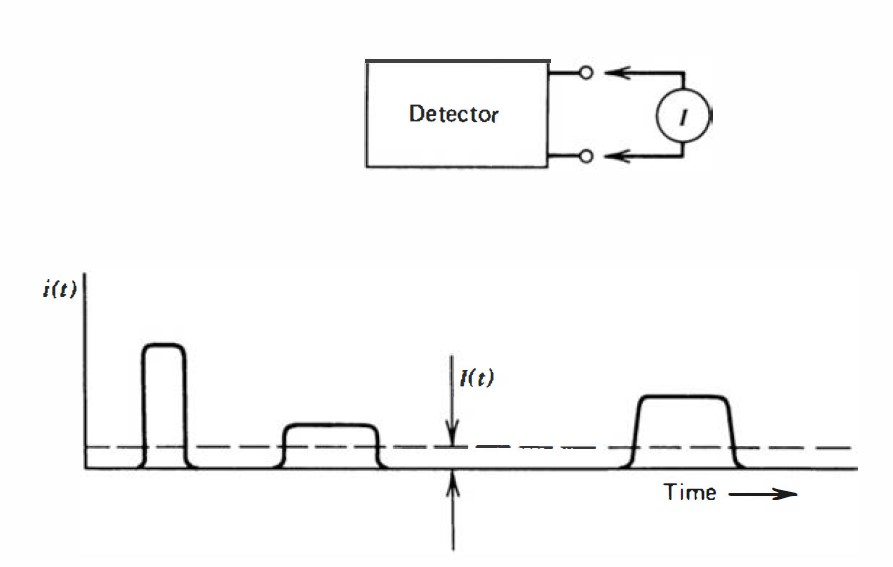
\includegraphics[width=0.7\textwidth]{Imagens/esquemaModoCorrente.jpg}
					\caption{Esquema de Detector Operando no Modo Corrente.}
					\label{fig:esquemaModoCorrente}
				\end{figure}
			
			No modo corrente, assume-se que o tempo de resposta T do detector é fixo, e portando diversos pulsos de corrente emitidos em um tempo t serão coletados ao longo do tempo de resposta do detector, gerando uma corrente dependente do tempo dada por:
			
				\begin{equation}
					I(t) = \frac{1}{T} \int_{t-T}^{t} i (t') \,dt' 
				\end{equation}

			\noindent Como o tempo de resposta T é muito maior que o intervalo de tempo entre os pulsos de corrente individuais, o efeito é compensar muitas das flutuações nos intervalos entre as interações individuais e registrar uma corrente média que depende do produto da taxa de interação e a carga média por interação.

			A corrente média é dada pelo produto da taxa de eventos com a média de carga produzida por cada evento; portanto:

				\begin{equation}
					I_0 = rQ = r\frac{E}{W}q
				\end{equation}
			
			\noindent onde:

				\begin{tabular}{l l l }
				r & = & Taxa de Eventos \\
				Q & = & carga produzida por cada evento \\
				E & = & energia média depositada por cada evento \\
				W & = & Energia média para produzir um par elétron-íon \\
				q & = & carga elétrica ($1.6 \times 10^{-19}C$)
				\end{tabular}

			Para uma irradiação estacionária do detector, a corrente média pode ser descrita como a soma da corrente constante $I_0$ com a componente de flutuação da corrente dependente do tempo ($\sigma_i(t)$), no qual é a variável aleatória dependente do tempo que ocorre como consequência da natureza aleatória dos eventos interagindo com o detector,  como mostra a figura \ref{fig:esquemaCorrenteFlutuacao}.

			\begin{figure}[h]
				\centering
				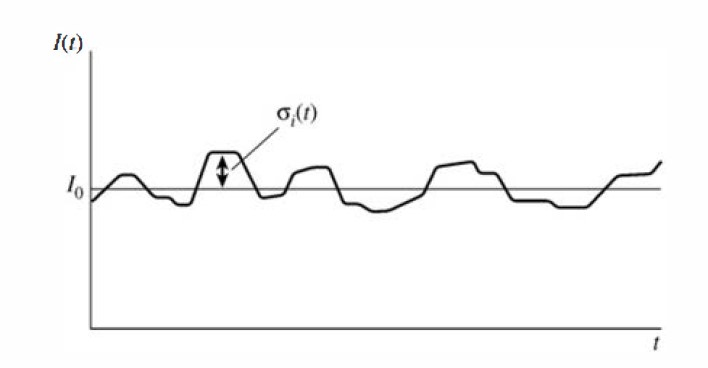
\includegraphics[width=0.7\textwidth]{Imagens/esquemaCorrenteFlutuação.jpg}
				\caption{Irradiação estacionária com flutuação}
				\label{fig:esquemaCorrenteFlutuacao}
			\end{figure}

		\subsubsection{Modo Pulso}

			A natureza do sinal produzido por um único evento depende das características de entrada do circuito no qual o detector está conectado, normalmente utilizando um pré-amplificador. A figura \ref{fig:esquemaModoPulso} apresenta um esquema básico de um circuito utilizado no modo pulso. 

				\begin{figure}[h]
					\centering
					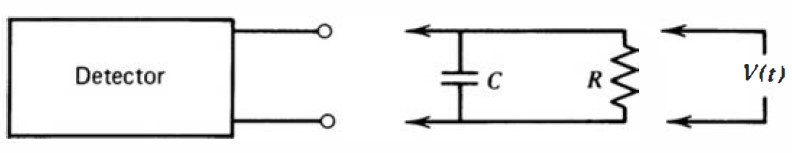
\includegraphics[width=0.8\textwidth]{Imagens/esquemaModoPulso.jpg}
					\caption{Circuitos de um detector operando em modo pulso}
					\label{fig:esquemaModoPulso}
				\end{figure}

			\noindent Onde R representa a resistência de entrada do circuito e C representa a capacitância equivalente que considera a capacitância do detector e do circuito de medição; Caso um pré-amplificador seja acoplado ao detector, então R será a resistência de entrada e C será a soma das capacitâncias do detector, do cabo que conecta o detector ao pré-amplificador e capacitância de entrada do próprio pré-amplificador. $V(t)$ é a tensão dependente do tempo, com o qual o modo pulso é baseado. 

			Resistência elétrica é a oposição que um material apresenta à passagem de corrente elétrica através dele. Essa oposição é causada pelos elétrons que compõem o material e que se movem em resposta a um campo elétrico aplicado, colidindo com outras partículas do material e transferindo energia para elas. 

			A resistência elétrica limita a quantidade de corrente elétrica que pode fluir através do circuito. A Lei de Ohm estabelece que a corrente elétrica que flui através de um material é diretamente proporcional à diferença de potencial elétrico aplicada (tensão) e inversamente proporcional à resistência elétrica do material, ou seja:

				\begin{equation}
					I = \frac{V}{R}
				\end{equation}

			\noindent Onde I é a corrente elétrica dada em amperes (A), V é a diferença de potencial dada em volts (V) e R é a resistência dada em ohms ($\omega$).

			A Capacitância é uma grandeza elétrica que mede a capacidade de um objeto de armazenar carga elétrica quando submetido a uma diferença de potencial elétrico e está envolvida em circuitos elétricos que possuem capacitores.
			
			Os capacitores são dispositivos eletrônicos que consistem em duas placas condutoras separadas por um material isolante (dielétrico). Quando uma tensão é aplicada ao capacitor, as cargas elétricas se acumulam nas placas, criando um campo elétrico entre elas. Esse campo elétrico é proporcional à carga elétrica armazenada no capacitor e inversamente proporcional à capacitância do capacitor.

			A capacitância é dada pela relação entre a carga elétrica armazenada e a diferença de potencial elétrico aplicada ao capacitor, dada por:

				\begin{equation}
					C = \frac{Q}{V}
				\end{equation}

			\noindent Onde C é a capacitância em farads (F), Q é a carga elétrica armazenada em coulombs (C) e V é a diferença de potencial elétrico (tensão) em volts (V) aplicada ao capacitor.
			
			Um circuito RC é um circuito elétrico composto por um resistor (R) e um capacitor (C) conectados em série ou em paralelo. A operação desse circuito depende da capacidade do capacitor de armazenar e liberar carga elétrica.

			Quando uma tensão é aplicada ao circuito, o capacitor começa a carregar. Durante esse processo, a corrente elétrica flui através do resistor, reduzindo a tensão aplicada ao capacitor. A taxa de carga depende do valor da resistência e da capacitância do circuito, conforme determinado pela constante de tempo.

			A constante de tempo em um circuito RC é um parâmetro que indica a rapidez com que um capacitor carrega ou descarrega em resposta a uma mudança na tensão aplicada a ele através de um resistor. É uma medida do tempo necessário para que a tensão do capacitor atinja aproximadamente 63,2\% do seu valor final após uma mudança na tensão de entrada.

			Após um certo tempo, o capacitor atinge seu limite de carga máxima e começa a armazenar energia elétrica. Se a tensão aplicada ao circuito for interrompida, o capacitor começa a descarregar através do resistor, liberando a energia armazenada. A taxa de descarga também depende do valor da resistência e da capacitância, conforme determinado pela constante de tempo.
			
			A constante de tempo para um circuito RC  é dada por:
			
				\begin{equation}
					\tau = R \cdot C
				\end{equation}

			\noindent onde $\tau$ é a constante de tempo em segundos, R é a resistência em ohms e C é a capacitância em farads. 
			
			A constante de tempo é importante em circuitos que envolvem a carga e descarga de capacitores, pois ela afeta a taxa de mudança da tensão no capacitor e, portanto, o comportamento do circuito como um todo.
			
			Pode-se então avaliar dois extremos de operação: Quando a constante de tempo do circuito é muito menor que o tempo para a coleta da carga e quando a constante de tempo é muito maior que o tempo para a coleta da carga.

			\begin{wrapfigure}{r}{0.5\textwidth}
				\centering
				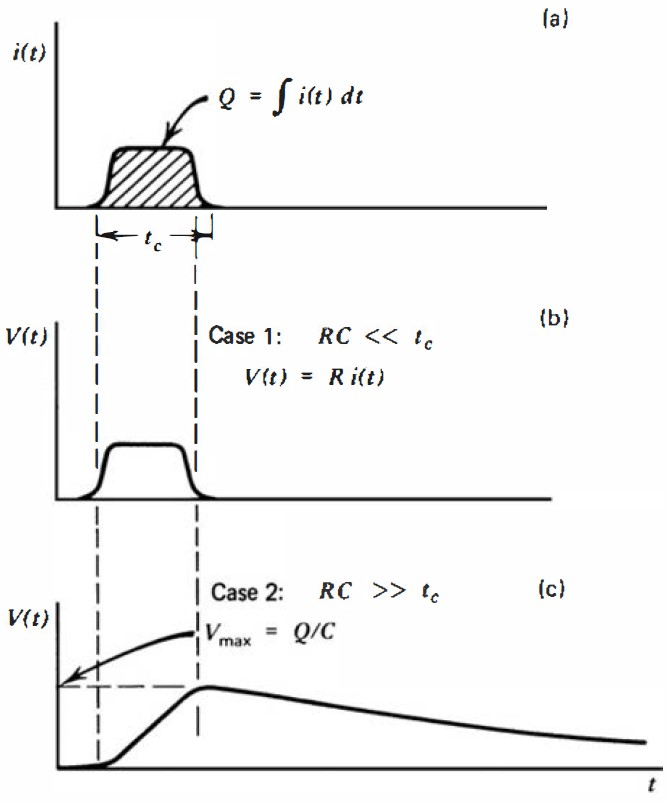
\includegraphics[width=0.41\textwidth]{Imagens/esquemaCorrentesCircuitoRC.jpg}
				\caption{Extremos de Operação}
				\label{fig:esquemaCorrenteCircuitoRC}
			\end{wrapfigure}


			$\tau \ll t_c$: Neste caso a constante de tempo do circuito externo é mantida pequena comparada ao tempo para coleta da carga, de forma que a corrente fluindo através da resistência R é essencialmente igual ao valor instantâneo da corrente fluindo no detector. O sinal da voltagem V(t) produzidos sob estas condições tem a forma aproximadamente idêntica à dependência temporal da corrente produzida dentro do detector, como mostra a figura \ref{fig:esquemaCorrenteCircuitoRC}(b). Os detectores de radiação as vezes operam sob estas condições quando informações a respeito de altas taxas de eventos ou informações temporais são mais importantes que uma informação precisa da energia.

			$\tau \gg t_c$: Este é o principal modo de operação dos detectores que operam no modo pulso. Neste caso a constante de tempo é mantida grande o suficiente quando comparada ao tempo de coleta da carga de modo que uma corrente muito pequena irá fluir através da resistência R durante o tempo de coleta da carga e a corrente do detector é momentaneamente integrada à capacitância. Se assumirmos que o tempo entre os pulsos é suficientemente grande, o capacitor começará a descarregar através da resistência, retornando a voltagem da resistência para zero, como mostra a Figura \ref{fig:esquemaCorrenteCircuitoRC} (c).


			\begin{itemize}
				\item O tempo necessário para o pulso do sinal alcançar seu valor máximo é determinado pelo tempo de coleção de carga dentro do próprio detector;
				\item O tempo necessário para restaurar a tensão do sinal para zero é determinado apenas pela constante de tempo do circuito elétrico.
				\item A amplitude do pulso de sinal é determinada pela seguinte relação:
					\begin{equation}
						V_{max} = \frac{Q}{C}
					\end{equation}
			\end{itemize}

			Portanto, o output de um detector operando em modo pulso consiste em uma sequência de pulsos de sinais individuais representando o resultado da interação de uma única partícula com o detector, e a amplitude de cada pulso individual reflete a quantidade de carga liberada nessa interação.

			Só existe uma proporcionalidade entre $V_{max}$ e a Carga $Q$ caso a capacitância se mantenha constante. Na maior parte dos detectores, a capacitância inerente é dada pela a forma e tamanho do capacitor utilizado no circuito de forma que é garantida uma capacitância constante. Em outros casos, como ocorre com os diodos semi-condutores, a capacitância pode mudar devido a uma variação nos parâmetros normais de operação. Nestes casos, pulsos de voltagem com diferentes amplitudes podem ser gerados a partir da mesma carga total liberada na interação Q. 

			Comparando os detectores operando em modo pulso com os detectores operando em modo corrente, podemos inferir que:

			\begin{itemize}
				\item A sensibilidade alcançada dos detectores operando no modo pulso é frequentemente muito maior que a sensibilidade dos detectores que operam no modo corrente, pois cada interação individual pode ser detectada como um pulso distinto.
				\item No modo pulso, os limiares de detecção são definidos a partir dos níveis de radiação de fundo; No modo corrente, a corrente mínima detectável pode representar uma taxa média de eventos muito maior que a radiação de fundo;
				\item No modo pulso, cara amplitude de pulso carrega alguma informação que é sempre útil ou uma parte necessária de uma aplicação em particular; Já no modo corrente, a informação a respeito da amplitude do pulso é perdida e todas as interações, independente da amplitude, contribuem para a corrente média medida. 
			\end{itemize}

	\subsection{Espectro de Altura de Pulso}

		Quando um detector opera no modo pulso, cada amplitude de pulso gerada carrega informação a cerca da carga gerada em cada interação; Porém, ao avaliar diversos pulsos, nota-se que as amplitudes nem sempre são as mesmas e isto se deve à diferenças de energias das partículas incidentes ou até mesmo flutuações inerentes à resposta do detector em feixes monoenergéticos. 

		A distribuição de amplitude de pulso pode ser utilizada para deduzir informações a respeito da radiação incidente ou para obter informações a respeito da operação do próprio detector. Estas distribuições podem ser exibidas na forma integral ou diferencial.



		\subsubsection*{Distribuição Diferencial de Altura de Pulso}

			A Figura \ref{fig:distribuicaoDeAlturaDePulso} (a) fornece uma distribuição hipotética onde: a abscissa é a escala linear de amplitude de pulso que vai de zero até o maior valor de amplitude observado para a fonte, fornecida em volts (V); O eixo das ordenadas representa o número diferencial $dN$  de pulsos observados para uma amplitude dentro de um incremento diferencial de amplitude $dH$, dividido por esse incremento, ou seja $dN/dH$, fornecido em \unit{V^{-1}}.

			O número de pulsos cuja amplitude está entre dois valores pré-determinados $H_1$ e $H_2$ podem ser obtidos através da área da curva limitada por estas duas amplitudes, ou seja:

				\begin{equation}
					N_{H_1 \rightarrow  H_2} = \int_{H_1}^{H_2} \frac{dN}{dH}  \,dH 
				\end{equation}

				\begin{wrapfigure}{l}{0.6\textwidth}
					\centering
					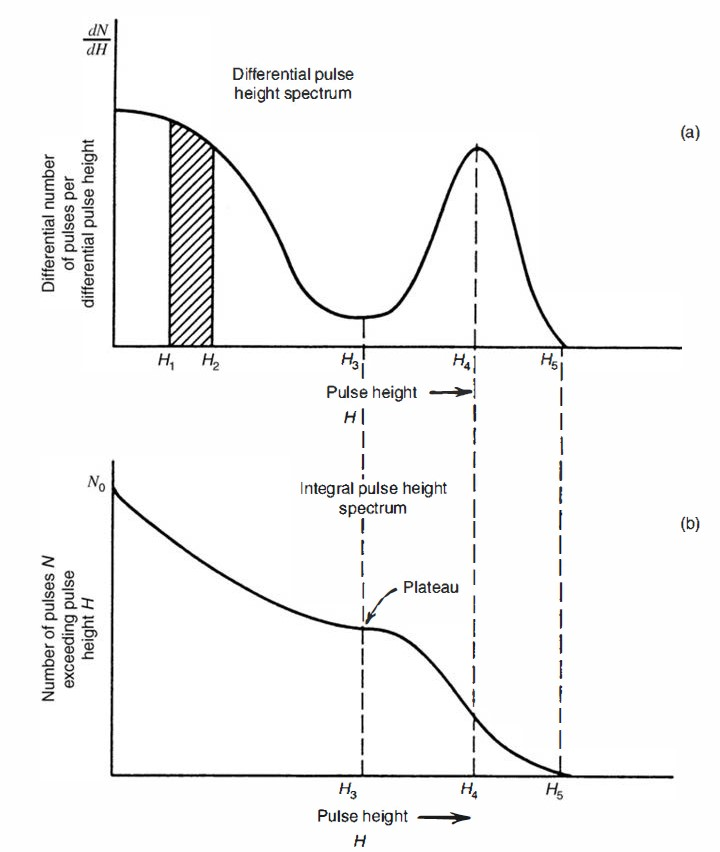
\includegraphics[width=0.59\textwidth]{Imagens/distribuicaoDeAlturaDePulso.jpg}
					\caption{Distribuições de Amplitude}
					\label{fig:distribuicaoDeAlturaDePulso}
				\end{wrapfigure}

			O número total de pulsos $N_0$ pode ser obtido através da área total embaixo da curva, ou seja:

				\begin{equation}
					N_0 = \int_{0}^{\infty} \frac{dN}{dH} \,dH
				\end{equation}

			A amplitude de pulso máxima observada ($H_5$) é o ponto ao longo da abscissa no qual a distribuição vai para zero; Picos na distribuição, como ocorre em $H_4$, indicam que são encontrados uma grande quantidade de pulsos para aquela amplitude de pulso; Os vales na distribuição, como ocorre em $H_3$, indicam que são encontrados poucos números de pulsos para aquela determinada amplitude de pulso. 

		\subsubsection*{Distribuição Diferencial de Altura de Pulso}

			A Figura \ref{fig:distribuicaoDeAlturaDePulso} (b) mostra a distribuição integral para o mesmo espectro apresentado na Figura \ref{fig:distribuicaoDeAlturaDePulso} (a). O eixo das abscissas também representa a escala de amplitude de pulso, e o eixo das ordenadas apresenta o número de pulsos N no qual a amplitude excede o valor apresentado no eixo das abscissas H. N diminui em função H pois cada vez menos pulsos estarão acima de uma amplitude $H_i$ que pode aumentar seu valor além de zero. 
			
			Como todos os pulsos possuem uma amplitude finita maior que zero, então $H = 0$ representa o número total de pulsos observados $N_0$ e a medida que H aumenta a N diminui até que a distribuição integral cai para zero na amplitude de pulso máxima observada ($H_5$). 


		A amplitude da distribuição diferencial, ou seja, o número de pulsos de qualquer amplitude de pulso H é dada pelo valor absoluto da curva da distribuição integral no mesmo valor H; Nos locais onde aparecem picos na distribuição diferencial, representam pontos de máximo local na distribuição integra; E semelhantemente, as regiões de vale na distribuição diferencial representa os mínimos locais de amplitudes de pulsos na distribuição integral. 


	\subsection{Curvas de Contagem e Platôs}

		Quando os detectores operam no modo de contagem pulsada, os pulsos do detector são enviados para um dispositivo de contagem que possui um nível fixo de discriminação, ou seja possui um limiar de amplitude de pulso. Para que um pulso de sinal seja registrado pelo circuito do contador este pulso deverá exceder um limiar de amplitude de pulso $H_d$. É possível variar o limiar $H_d$ durante a medição afim de se obter informações a cerca da distribuição de amplitudes de pulso, e medidas realizadas com estas variações resultará da distribuição integral de amplitudes de pulso. 

		Ao realizar uma medida de contagem, a medição deverá ser configurada de modo que se estabeleça um ponto de operação no qual irá ser alcançada a maior estabilidade sob longos períodos de tempo. Ou seja, durante uma medição podem ocorrer pequenos desvios em $H_d$ e portanto deve ser estabelecido um ponto de operação que fará com que esse desvio tenha influência mínima na contagem medida. Como mostra a Figura \ref{fig:distribuicaoDeAlturaDePulso}, o ponto em $H_3$ se configura como um ponto estável de operação; Este ponto representa o ponto de mínimo global da distribuição diferencial de forma que representa um ponto com  variação mínima na curva integral, portanto pequenos desvios no limiar $H_d$ terão um impacto mínimo no número total de pulsos registrados. No geral, regiões de mínimo na curva integral são chamados de platô de contagem e representam áreas de operação no qual é possível alcançar uma sensibilidade mínima a variações no limiar de amplitude. 

		O platô em contagem de dados também é observado em processos no qual a carga produzida a cada interação é aumentada para um determinado detector de radiação; onde muitas vezes é possível variar o ganho ou a amplificação fornecida para a carga produzida na interação. Esta variação pode ser feita alterando o fator de amplificação de um amplificador linear posicionado entre o detector e o circuito de contagem, ou pode ser feita diretamente alterando a voltagem aplicada no próprio detector. 

		A Figura \ref{fig:curvaContagemGanho} (a) apresenta uma distribuição diferencial de amplitude de pulso, para três valores diferentes de ganho da voltagem. Neste caso, o valor do ganho (G) pode ser definido como a razão entre a amplitude da voltagem para um dado evento no detector e a mesma amplitude antes de algum parâmetro ser alterado, como o fator de amplificação ou a voltagem do detector. 

			\begin{figure}[h]
				\centering
				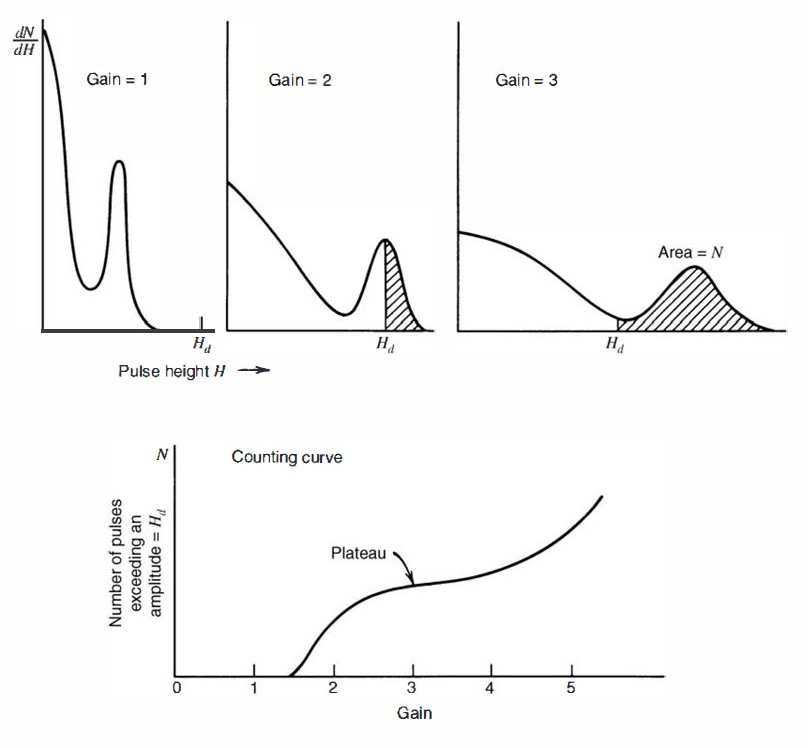
\includegraphics[width=0.8\textwidth]{Imagens/curvaContagemGanho.jpg}
				\caption{Exemplo de uma curva de contagem gerada através da variação do ganho mantendo as condições da fonte constante}
				\label{fig:curvaContagemGanho}
			\end{figure}

		
		Ao manter a irradiação constante, quanto maior o ganho na voltagem maior será a amplitude de pulso máxima, porém em ambos os casos a área sob a curva diferencial se manterá constante, ou seja, o número total de pulsos  será sempre o mesmo. A Figura \ref{fig:curvaContagemGanho} mostra que para o ganho G = 1, nenhuma contagem será registrada pois todas as amplitudes de pulso estão abaixo do limiar de amplitude para detecção. Ao realizar contagens em função do ganho da voltagem, obtem-se a distribuição integral, chamada de curva de contagens, apresentada na Figura \ref{fig:curvaContagemGanho} (b). Devido à pequenos valores de ganho, nenhum pulso é contado, porem a medida que o ganho é aumentado, aumenta-se o número de pulsos contados até que o ganho seja suficiente para contar todos os pulsos. 

		O platô na curva de contagem pode ser previsto com base no valor de ganho que faz com que o limiar de amplitude $H_d$ coincida aproximadamente com um ponto de mínimo na curva diferencial. 


	\subsection{Resolução de Energia}

		Diversas aplicações de detectores de radiação tem como objetivo medir a distribuição de energia da radiação incidente, chamado de forma geral como espectroscopia da radiação. A Figura \ref{fig:funcoesDeResposta} ilustra a distribuição diferencial de amplitude de pulso produzida por um detector submetido a um feixe monoenergético; Esta distribuição é chamada de \textbf{função resposta} de um detector para a energia utilizada na sua determinação. A curva chamada de ``Boa Resolução'' ilustra uma possível distribuição em torno da amplitude média de pulso $H_0$; A curva chamada de ``Baixa Resolução'', ilustra a resposta de um detector com um desempenho inferior. Desde que ambos os casos registrem o mesmo número de pulsos, as áreas embaixo das curvas são iguais.

		\begin{figure}[h]
			\centering
			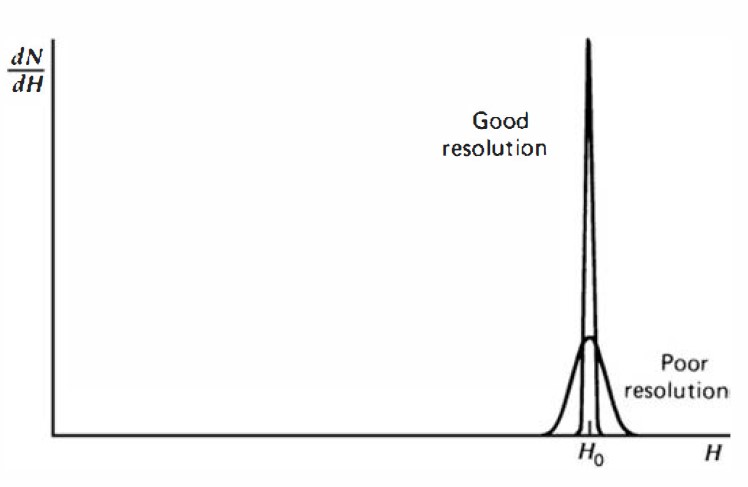
\includegraphics[width=0.7\textwidth]{Imagens/funcoesDeResposta.jpg}
			\caption{Funções de Resposta}
			\label{fig:funcoesDeResposta}
		\end{figure}

		Embora ambas as distribuições estejam centradas em torno do valor médio $H_0$, a largura da distribuição para a baixa resolução é muito maior. Esta largura reflete o fato de que foi registrada uma grande quantidade de flutuação de pulso a pulso embora a mesma energia tenha sido depositada para cada evento. Se a quantidade destas flutuações é for cada vez menor, a largura da distribuição será cada vez menor e a forma da curva se aproximará para uma função delta de dirac. 

		A definição para a resolução de energia de um detector pode ser observada na Figura \ref{fig:resolucaoDeEnergia}, onde a distribuição diferencial de amplitude de pulso é determinada para um detector submetido a um feixe monoenergético. 

			\begin{figure}[h]
				\centering
				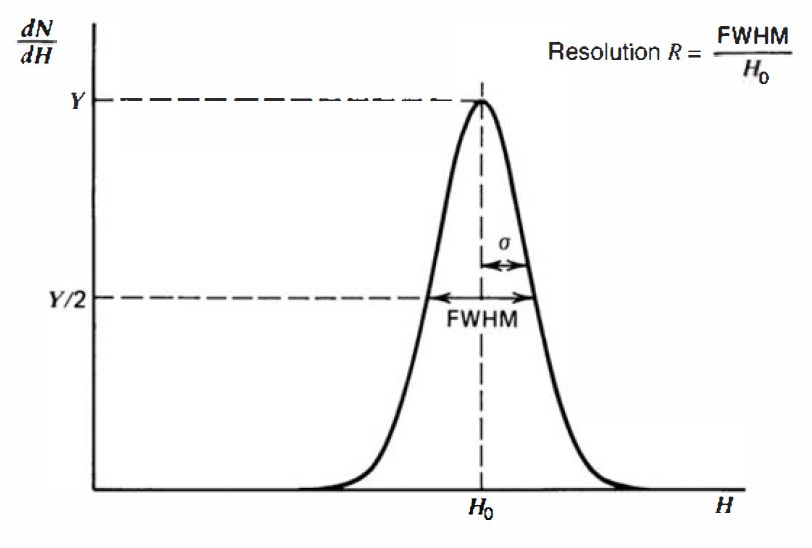
\includegraphics[width=0.7\textwidth]{Imagens/resolucaoDeEnergia.jpg}
				\caption{Resolução de Energia}
				\label{fig:resolucaoDeEnergia}
			\end{figure}


		A largura à meia altura (FWHM,  do inglês \textit{Full Width at Half Maximum}) é definida como a largura da distribuição na metade da altura do pico relacionado a $H_0$. Esta definição assume que qualquer sinal de fundo ou qualquer sinal contínuo que possa sobrepor o pico é negligenciável ou foi subtraído do sinal do pico. A resolução R é uma grandeza adimensional, e  sua fração é convencionalmente expressa em percentual. Um diodo possui resolução energética de aproximadamente 1\% enquanto que detectores cintiladores possuem uma resolução energética variando entre ~3\% até ~ 10\%.

		Quanto menor o valor para a resolução de energia, melhor será a habilidade do detector distinguir duas radiações cujas energias estão próximas uma da outra. Uma regra prática é que o detector deve ser capaz de detectar duas energias separadas por mais de uma FWHW .

		Algumns fatores que causam flutuações na resposta de um detector são: desvios nas características de operação do detector durante a medição; fontes de ruídos aleatórias dentro do detector e do sistema de instrumentação e o ruído estatístico proveniente da natureza discreta do próprio sinal medido. 
		
		O ruído estatístico representa a quantidade mínima de flutuação que não pode pode ser removida independente da qualidade do sistema de medição utilizado. O ruído estatístico surge devido ao fato de que a carga Q gerada dentro do detector devido a um quanta de radiação  não é uma variável contínua, mas sim um valor discreto do número de portadores de carga. Pode ser feita uma estimativa da flutuação inerente da detecção assumindo que os portadores de carga criados se se aproximam de distribuição Gaussiana.

	\subsection{Eficiência de Detecção}

		A eficiência de detecção varia com o tipo de radiação para o qual o detector será utilizado, sendo diferente para radiações diretamente ionizantes e indiretamente ionizantes.

		Quando uma radiação diretamente ionizante, como as partículas alfa e os elétrons, entra na cavidade do detector, causarão imediatamente ionizações e excitações no volume da cavidade, e após viajar uma pequena fração do seu alcance será liberado pares de íons suficientes que farão com que o pulso resultante seja grande o suficiente para ser registrado; Portanto, garantindo que o detector consiga detectar toda partícula carregada que entra em sua cavidade, pode-se dizer que o detector possuirá uma eficiência de contagem de 100\%. 

		Enquanto que a radiação diretamente ionizante é imediatamente detectada entrar na cavidade do detector, para detectar uma radiação indiretamente ionizante, ela deve primeiramente sofrer uma interação significante no detector, para então ser possível detectá-la. Como estas radiações podem viajar largas distâncias entre as interações, alguns quantas dessa radiação não serão detectados e portanto a eficiência do detector será sempre menor que 100\%.

		A eficiência na contagem é dividida entre:

			\begin{itemize}
				\item Eficiência Absoluta ($\epsilon_{abs}$), que é definida como a razão entre o número de pulsos registados $N_P$ e o número de partículas $N$ emitidas pela fonte, ou seja
				
					\begin{equation}
						\epsilon_{abs} = \frac{N_P}{N}
					\end{equation}
				
				A eficiência absoluta depende das propriedades do detector e da geometria  utilizada na contagem, sendo a principal componente a distância da fonte ao detector.
				
				\item Eficiência Intrínseca ($\epsilon_{int}$), que é definida como a razão entre o número de pulsos registrados $N_P$ e o Número de partículas $N_{in}$ que incidem no detector, ou seja:
				
					\begin{equation}
						\epsilon_{int} = \frac{N_P}{N_{in}}
					\end{equation}

				A eficiência intrínseca depende principalmente do material do detector, da energia da radiação, e da espessura de material do detector na região de incidência do feixe. 
			\end{itemize}

		A relação entre as eficiências para uma fonte isotrópica é dada por:

			\begin{equation}
					\epsilon_{int} = \epsilon_{abs} \cdot \left(\frac{4 \pi}{\Omega}\right)
			\end{equation}

		\noindent onde $\Omega$ é o ângulo sólido do detector visto a partir da posição da fonte.

	\subsection{Tempo Morto}

		Praticamente todos os detectores necessitam de uma quantidade de tempo mínima entre dois eventos para que ele possa registrar separadamente os dois pulsos, e essa limitação pode estar relacionada com a forma em si de realizar a detecção ou devido aos componentes eletrônicos do detector. Devido a natureza aleatória do decaimento radioativo, sempre existirá a possibilidade de um sinal verdadeiro não ser registrado por ocorrer muito próximo a outro evento. 

	\section{Câmaras de Ionização}

		

	
\bibliography{ref.bib}
\end{document}